\documentclass[10pt,twocolumn,letterpaper]{article}

\usepackage{iccv}
\usepackage{times}
\usepackage{epsfig}
\usepackage{graphicx}
\usepackage{amsmath}
\usepackage{amssymb}
\documentclass[10pt,twocolumn,letterpaper]{article}

\usepackage{iccv}
\usepackage{times}
\usepackage{epsfig}
\usepackage{graphicx}
\usepackage{amsmath}
\usepackage{amssymb}
\usepackage{graphicx}

% ------ New Package Here ------
\usepackage{dblfloatfix}
\usepackage{subcaption}
\usepackage{bm}
\usepackage[pagebackref=true,breaklinks=true,letterpaper=true,colorlinks=true,bookmarks=true]{hyperref}
% ------------------------------

\makeatletter
\newcommand\footnoteref[1]{\protected@xdef\@thefnmark{\ref{#1}}\@footnotemark}
\makeatother


%---------MATH SYMBOLS NEW COMMANDS:--------------------------------------
\newcommand{\vectornorm}{|}

\newcommand{\diver}{\mathrm{div}}
\newcommand{\grad}{\mathrm{grad}}
\newcommand{\trace}{\mathrm{trace}}
\newcommand{\ud}{\mathrm{d}}

\newcommand{\mvec}[1]{\boldsymbol{#1}}
\newcommand{\matr}[1]{\mathrm{#1}}

\newcommand{\eye}{\mathrm{I}}
\newcommand{\img}{u}

\newcommand{\prob}[1]{\mathrm{p}\left( #1 \right)}

\newcommand{\bhat}{\widehat{\mvec{b}}}
\newcommand{\lamhat}{\widehat{\mvec{\lambda}}}
\newcommand{\eps}{\mvec{\varepsilon}}

%\newcommand{\norm}[1]{\left\Vert#1\right\Vert}
% \newcommand{\norm}[1]{\left \|#1 \right \|}
\newcommand{\norm}[1]{\left |#1 \right |}
\newcommand{\transp}{^\mathrm{T}}

\newcommand{\bu}{\boldsymbol{u}}
\newcommand{\bx}{\boldsymbol{x}}
\newcommand{\bp}{\boldsymbol{p}}

\newcommand{\be}{\boldsymbol{\varepsilon}}

\newcommand{\bv}{\boldsymbol{v}}
\newcommand{\mfsf}[0]{{\sc mfsf}}
\newcommand{\mfsfc}[0]{{\sc mfsf\em c}}
\newcommand{\mfsfdct}[0]{{\sc mfsf$_{\tt DCT}$}}
\newcommand{\mfsfpca}[0]{{\sc mfsf$_{\tt PCA}$}}
\newcommand{\mfsfid}[0]{{\sc mfsf$_{\tt I_{2F}}$}}
\newcommand{\mfsfcdct}[0]{{\sc mfsf\em c$_{\tt DCT}$}}
\newcommand{\mfsfcpca}[0]{{\sc mfsf\em c$_{\tt PCA}$}}
\newcommand{\mfsfcid}[0]{{\sc mfsf\em c$_{\tt I_{2F}}$}}


\newcommand{\cU}{\mathcal{U}}
\newcommand{\bU}{\boldsymbol{\mathcal{U}}}
\newcommand{\bE}{\boldsymbol{\mathcal{E}}}
\newcommand{\bI}{\boldsymbol{I}}
\newcommand{\bA}{\boldsymbol{A}}
\newcommand{\bb}{\boldsymbol{b}}
\DeclareMathOperator*{\argmin}{arg\,min}
\DeclareMathOperator*{\argmax}{arg\,max}


\newcommand{\bL}{\boldsymbol{L}}
\newcommand{\bM}{\boldsymbol{M}}

\newcommand{\R}{\mathbb{R}}

\newcommand{\Lone}{\mathbf{L}^1}
\newcommand{\Ltwo}{\mathbf{L}^2}


%----------------------------------------------------------------------------------------------------

% Include other packages here, before hyperref.

% If you comment hyperref and then uncomment it, you should delete
% egpaper.aux before re-running latex.  (Or just hit 'q' on the first latex
% run, let it finish, and you should be clear).
\usepackage[pagebackref=true,breaklinks=true,letterpaper=true,colorlinks,bookmarks=false]{hyperref}


% \iccvfinalcopy % *** Uncomment this line for the final submission

\def\iccvPaperID{****} % *** Enter the ICCV Paper ID here
\def\httilde{\mbox{\tt\raisebox{-.5ex}{\symbol{126}}}}

% Pages are numbered in submission mode, and unnumbered in camera-ready
\ificcvfinal\pagestyle{empty}\fi
\begin{document}

%%%%%%%%% TITLE
\title{Constructing Statistical Deformable Models with Shape Flow}

\author{Yuxiang Zhou, Joan Alabort-i-Medina, Anastasios Roussos, Stefanos Zafeiriou\\
Imperial College London\\
180 Queen’s Gate, SW7 2AZ, London, U.K.\\
{\tt\small \{yuxiang.zhou10, ja310, troussos, s.zafeiriou\}@imperial.ac.uk}}
% For a paper whose authors are all at the same institution,
% omit the following lines up until the closing ``}''.
% Additional authors and addresses can be added with ``\and'',
% just like the second author.
% To save space, use either the email address or home page, not both


\maketitle
% \thispagestyle{empty}

%%%%%%%%% ABSTRACT
\begin{abstract}
    % Uses Abstract from Nondas' paper "Automatic Construction of Deformable Models In-The-Wild" as place holder with some modification. 
% Deformable objects are everywhere. Faces, ears, bodies,
% bottles etc. Recently, there has been a wealth of research
% on training deformable models for object detection,
% part localization and recognition using annotated data. In
% order to train deformable models with good generalization
% ability, a large amount of carefully annotated data is required,
% which is a highly time consuming and costly task.

% We propose the first - to the best of our knowledge - method
% for construction of dense deformable models using images
% captured in totally unconstrained conditions, recently
% referred to as “in-the-wild”. The only requirements of the
% method are drawings of image features. The object detector can be as simple as the
% Viola-Jones algorithm (e.g. even the cheapest digital camera
% features a robust face detector). The 2D shape model
% can be created by using only a few shape examples with deformations.
% In our experiments on facial deformable models,
% we show that the proposed automatically built model
% not only performs well, but also outperforms discriminative
% models trained on carefully annotated data. To the best of
% our knowledge, this is the first time it is shown that an automatically
% constructed model can perform as well as methods
% trained directly on annotated data.

Building and training deformable models of objects (e.g. faces, ears, bottles and cars) has  recently been widely researched for object detection, part localisation, fitting, recognition and tracking using manual annotated data. To train deformable models with satisfiable generalisation, large amount of carefully manual annotation is required. However, landmark annotation is extremely time consuming, work intensive and, most importantly, number of landmarks have to stay consistent for all training data while it is challenging to maintain the consistency or to avoid bias when annotating objects that having reach features like ears. We propose framework to handle training data with inconsistent annotation, build dense shape model and introduce effective curve annotation methods. In our experiment, we show building dense models trained with inconsistent annotation and trained with curve annotation improves performance of discriminative models trained on carefully annotated data.
\end{abstract}

%%%%%%%%% BODY TEXT
\section{Introduction}
    % Building and training deformable models of objects (e.g. faces, ears, bodies, bottles, vehicles etc.) has recently been widely researched for object detection, part localisation, fitting, recognition and tracking using manual annotated data. Shapes and appearances of majority of objects vary significantly from object instance. To illustrate, ears have complicated inner structures (e.g. helix, crus antihelicis, scapha, tragus, lobe etc.) which differs remarkably between ears and highly sensitive to intensity changes. Recently, we have witnessed a great progress in object detection, alignment and recognition. 

% To train deformable models with satisfiable generalisation, large amount of careful manual annotation is required. However, landmark annotation is extremely time consuming, work intensive and, most importantly, number of landmarks have to stay consistent for all training data while it is challenging to maintain the consistency or to avoid bias when annotating objects that having reach features. In ears, for example, large amount of landmarks required as the inner structure of ears are complex. To annotate an ear with clear contour, helix and cavum conchae, more than 50 landmarks are required. The inconsistency of ear features enhanced the difficulty of accurate annotation (e.g. Fossa Triangularies and Crus Helicis are optional feature of an ear also their visibility is highly sensitive to pose and illumination variation).
% To illustrate how much time consuming careful ear annotation is, according to our experience, a trained annotator may need an average of (TODO: experiment) minutes per image for the manual annotation of 55 landmarks. This means that the annotation of 1000 images requires a total of about (TODO: experiment). Furthermore, personal issue, prior knowledge and circumstances can heavily bias the annotation accuracy thus second round correction might desired.

% We propose a framework to (1) construct SDMs using training data with inconsistent annotation, (2) introduce highly effective curve annotation which tremendously reduces manual work overload but maintains same performance level against state-of-the-art SDMs and (3) build dense correspondent SDMs with shape flow. 

% %(1)
% Annotated data of same objects can have various number of landmarks, \cite{?} shown faces have landmarks different in range 10+ to 70+. Building SDMs (e.g. Active Appearance Models), however, require training data are annotated consistently, for example, all faces have 68 landmarks, 6 landmarks for an eye and 9 for a nose \cite{?}. Such property of SDMs largely limited their application area like combining different dataset as one. We propose the pipeline with non-rigid alignment and support vector shape to blend landmarks into relatively consistent shape discriminator before building models.

% %(2)
% Due to the fact that manual annotation is a rather costly and labour-intensive procedure, unsupervised and semi supervised learning of models for the tasks of alignment, landmark localization, tracking and recognition has attracted considerable attention \cite{?}. As our proposed framework are available to handle landmarks with inconsistency, it leads to a more efficient, convenient, unbiased and simple annotation methods - curve annotation. 

% %(3)
% To build dense correspondence between independent shapes, we apply optical flow on shapes with low rank constrains, so we name it shape flow. Optical flow is originally applied to video sequences that several assumptions holds, illumination consistency and motion smoothness, while shapes having no motion smoothness completely as all training data are independent. Low rank constrain plays important role to simulate motion smoothness assumption. 


% % Back Ground, uses Nondas' paper "Automatic Construction of Deformable Models In-The-Wild" as place holder
% The two most closely related works to the proposed
% method are the automatic construction of Active Appearance
% Models (AAMs) in \cite{?} and the so-called RASL
% methodology in \cite{?} for person-specific face alignment.
% There are two main differences between our framework
% and \cite{?}. (1) We use a predefined statistical shape model
% instead of trying to find both the shape and appearance models.
% We believe that with the current available optimization
% techniques, it is extremely difficult to simultaneously optimize
% for both the texture and shape parameters. (2) We
% employ the robust component analysis of \cite{?} for the appearance
% which deals with outliers. Thus, even though
% our method is similar in concept to \cite{?}, these two differences
% make the problem feasible to solve. In particular, the
% methodology in \cite{?} fails to create a generic model even in
% controlled recording conditions, due to extremely high dimensionality
% of the parameters to be found and to the sensitivity
% of the subspace method to outliers. This was probably
% one of the reasons why the authors demonstrate very
% limited and only person-specific experiments. Furthermore,
% our methodology bypasses some of the limitations of \cite{?},
% which requires the presence of only one low-rank subspace,
% hence it has been shown to work only for the case of congealing
% images of a single person. Finally, we argue that
% in order for an automatically constructed AAM methodology
% to be robust to both within-class and out-of-class outliers4,
% which cannot be avoided in totally unsupervised setting
% statistical component analysis techniques should be
% employed \cite{?}. 

% We summarize our contributions as follows:
% \begin{itemize}
%   \item Constructing SDMs using training data with inconsistent annotation.
%   \item Introduce highly effective curve annotation which tremendously reduces manual work overload but maintains same performance level against state-of-the-art SDMs.
%   \item Building dense correspondent SDMs with shape flow
% \end{itemize}

% In our experiment, we show that building robust dense models trained with inconsistent annotation and trained with curve annotation improves performance of discriminative models trained on carefully annotated data including ears, faces, bottles, (cars ?) and bodies. Evaluation methods and choices are described in details.


% \clearpage
\begin{figure}[t!]
    \centering
    \begin{subfigure}[b]{0.145\textwidth}
            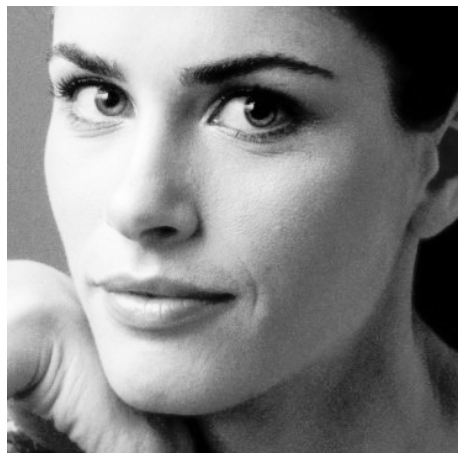
\includegraphics[width=\textwidth]{resources/intro_0_0}
    \end{subfigure}
    \hfill
    \begin{subfigure}[b]{0.145\textwidth}
            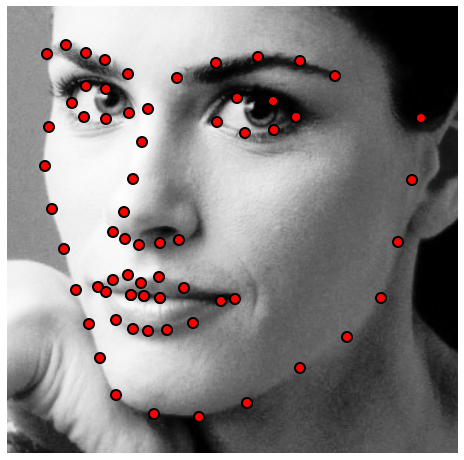
\includegraphics[width=\textwidth]{resources/intro_0_1}
    \end{subfigure}
   	\hfill
    \begin{subfigure}[b]{0.145\textwidth}
            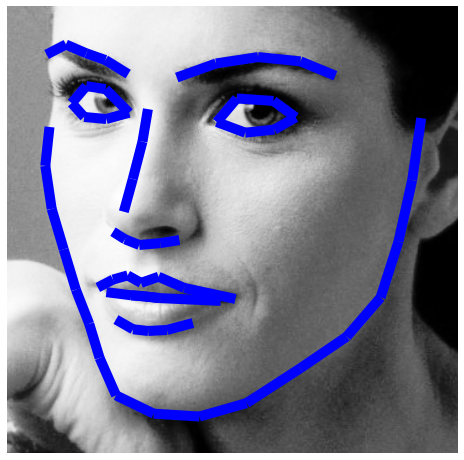
\includegraphics[width=\textwidth]{resources/intro_0_2}
    \end{subfigure}
    \\
    \begin{subfigure}[b]{0.075\textwidth}
            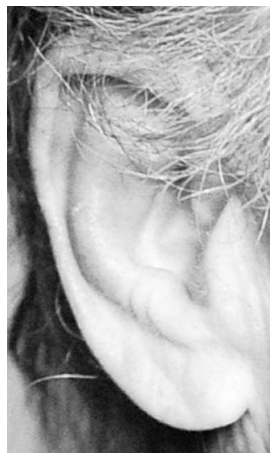
\includegraphics[width=\textwidth]{resources/intro_1_0}
    \end{subfigure}
    \hfill
    \begin{subfigure}[b]{0.075\textwidth}
            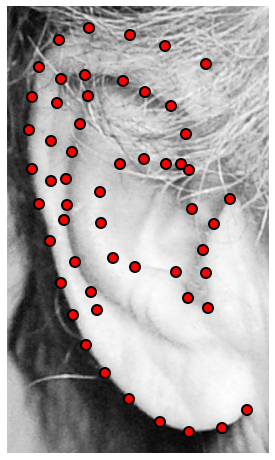
\includegraphics[width=\textwidth]{resources/intro_1_1}
    \end{subfigure}
   	\hfill
    \begin{subfigure}[b]{0.075\textwidth}
            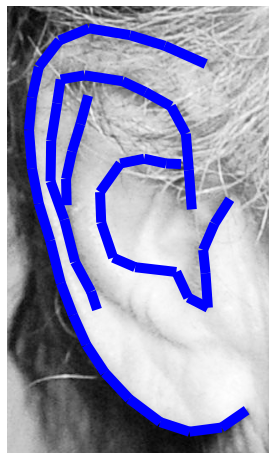
\includegraphics[width=\textwidth]{resources/intro_1_2}
    \end{subfigure}
    \hfill
    \begin{subfigure}[b]{0.075\textwidth}
            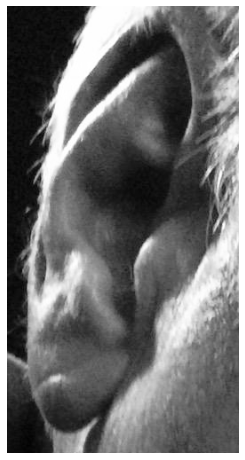
\includegraphics[width=\textwidth]{resources/intro_1_3}
    \end{subfigure}
    \hfill
    \begin{subfigure}[b]{0.075\textwidth}
            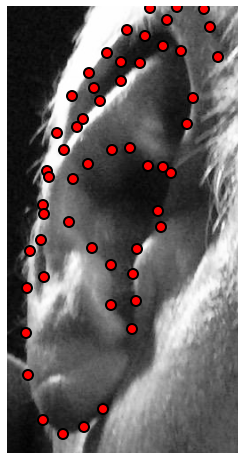
\includegraphics[width=\textwidth]{resources/intro_1_4}
    \end{subfigure}
   	\hfill
    \begin{subfigure}[b]{0.075\textwidth}
            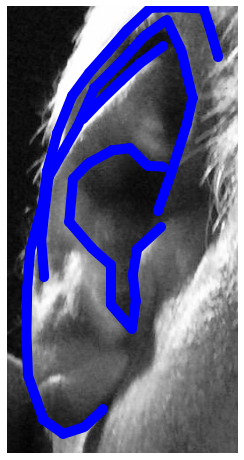
\includegraphics[width=\textwidth]{resources/intro_1_5}
    \end{subfigure}
    \\
    \begin{subfigure}[b]{0.07\textwidth}
            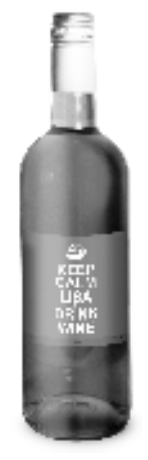
\includegraphics[width=\textwidth]{resources/intro_2_0}
    \end{subfigure}
    \hfill
    \begin{subfigure}[b]{0.07\textwidth}
            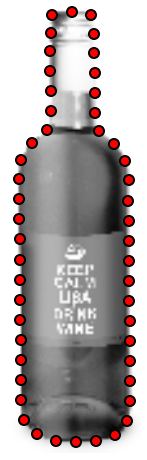
\includegraphics[width=\textwidth]{resources/intro_2_1}
    \end{subfigure}
   	\hfill
    \begin{subfigure}[b]{0.07\textwidth}
            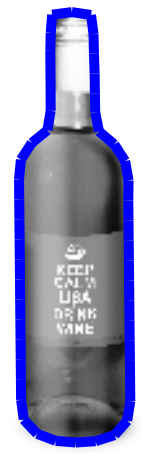
\includegraphics[width=\textwidth]{resources/intro_2_2}
    \end{subfigure}
    \hfill
    \begin{subfigure}[b]{0.07\textwidth}
            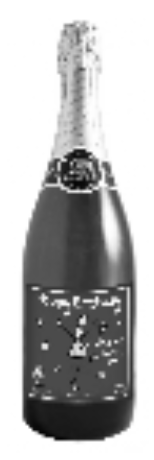
\includegraphics[width=\textwidth]{resources/intro_2_3}
    \end{subfigure}
    \hfill
    \begin{subfigure}[b]{0.07\textwidth}
            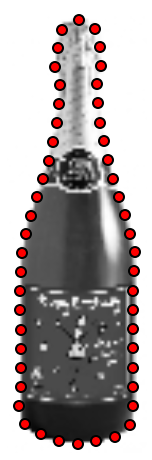
\includegraphics[width=\textwidth]{resources/intro_2_4}
    \end{subfigure}
   	\hfill
    \begin{subfigure}[b]{0.07\textwidth}
            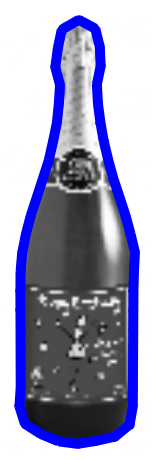
\includegraphics[width=\textwidth]{resources/intro_2_5}
    \end{subfigure}
    \\
    \begin{subfigure}[b]{0.075\textwidth}
            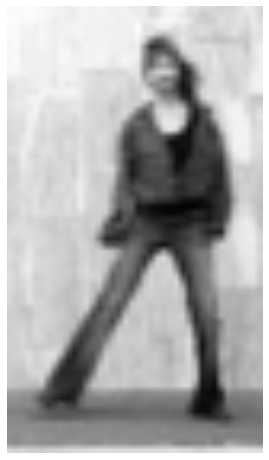
\includegraphics[width=\textwidth]{resources/intro_3_0}
    \end{subfigure}
    \hfill
    \begin{subfigure}[b]{0.075\textwidth}
            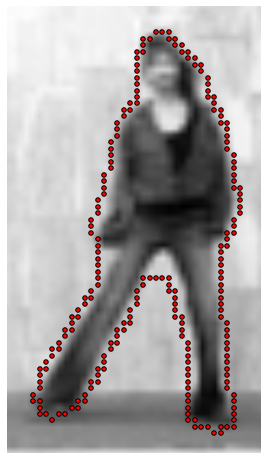
\includegraphics[width=\textwidth]{resources/intro_3_1}
    \end{subfigure}
   	\hfill
    \begin{subfigure}[b]{0.075\textwidth}
            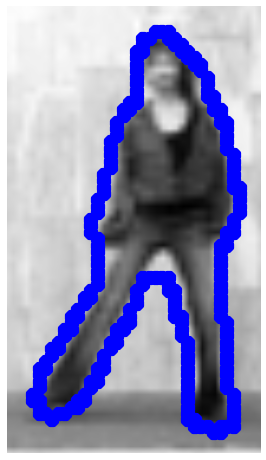
\includegraphics[width=\textwidth]{resources/intro_3_2}
    \end{subfigure}
    \hfill
    \begin{subfigure}[b]{0.075\textwidth}
            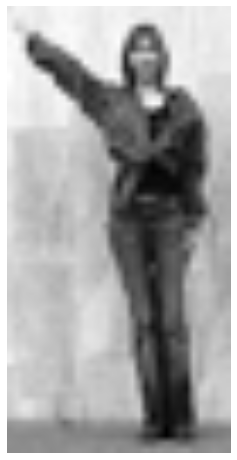
\includegraphics[width=\textwidth]{resources/intro_3_3}
    \end{subfigure}
    \hfill
    \begin{subfigure}[b]{0.075\textwidth}
            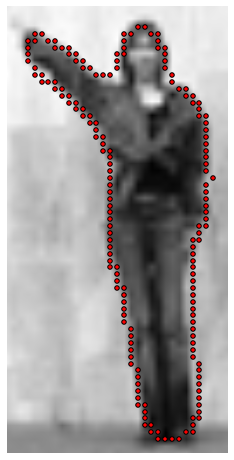
\includegraphics[width=\textwidth]{resources/intro_3_4}
    \end{subfigure}
   	\hfill
    \begin{subfigure}[b]{0.075\textwidth}
            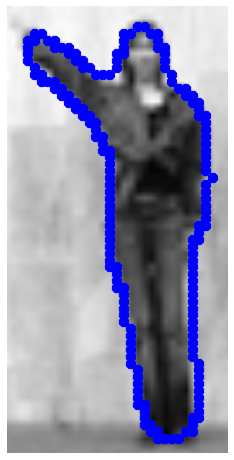
\includegraphics[width=\textwidth]{resources/intro_3_5}
    \end{subfigure}
    \caption{Figure}
\end{figure}

Building and fitting statistical deformable models of objects is a well-studied and popular area in the intersection of computer vision and machine learning [..]. Recently, we have witnessed tremendous developments in building and fitting models of human face and body using images captured in unconstrained recording conditions, usually referred to as "in-the-wild" [..]. This is attributed to 
\begin{itemize}

\item the abundance of complex visual data, spread mostly through the internet via web services such as Youtube, Flickr and Google Images. The latter has led to the development of huge databases of "in-the-wild" images of human faces and bodies [..]. Equally important is the task of manual annotation of images with regards to face and body parts and that has been undertaken by several research teams [..].

\item the development of powerful visual features, able to describe objects and its parts in a robust manner (e.g., Scale Invariant Feature Transforms (SIFT) [39], Histogram of Oriented Gradients (HoGs) [16] and recently Deep Convolutional Neural Networks [..]), as well as generative and discriminative methodologies for learning deformable models. 

\end{itemize}

There are two drawbacks on building deformable models that rely on landmarks 
\begin{itemize}

\item annotating with regards to consistent landmark annotation is extremely time consuming, laborious and labour intensive work [..], which usually can be performed by a trained person. Furthermore, for many objects it requires a highly skilled person to identify and annotate a set of images with regards to a consistent set of landmarks. For example human ears have very complicated inner structures (e.g. helix, crus antihelicis, scapha, tragus, lobe etc.) which differs remarkably between ears. Furthermore, 
certain ear parts, such as  Fossa Triangularies and Crus Helicis, do not appear in all ears and  their visibility is highly sensitive to pose and illumination variation. Please see Fig... 

\item the nature of many deformable objects do not allow to be consistently annotated with regards to a set of landmarks (e.g. bottles, fruits etc.). Also the boundary/outline of objects, such as faces, ears, body can be very difficultly annotated consistently. That is why many state-of-the-art opt to leave the boundary out for comparison [..]. An example is given in Fig.. The majority of the state-of-the-art methods for landmark-based deformable models [..] are not applicable for objects with no consistent set of landmarks. 

\end{itemize}

To illustrate how time consuming careful annotation of ears is we lay down our own experience. A trained annotator needs an average of 4 minutes per image for the manual annotation of 55 landmarks. This means that the annotation of 1000 images requires a total of about 67 hours. Furthermore,  training and fatigue largely influence the annotation accuracy. Hence, a second pass on the annotated data is, in many cases, necessary. Due to the fact that manual annotation is a rather costly and labour-intensive procedure, unsupervised learning of deformable models for the tasks of alignment has recently attracted some attention \cite{?}. Nevertheless, the method [..] requires a consistent set of shapes annotated with landmarks to perform deformable face congealing. Finally, since the problem of fully unsupervised discovery of the deformations of arbitrary objects is a very difficult and ill-posed problems the limited number of methods [..] that have been applied for the task cannot be applied for arbitrary collection of images collected "in-the-wild". 


In this paper, we provide a solution for annotating an object with regards to its deformations that requires considerable less effort and in the same time can be used to define statistical deformations for objects without consistent set of landmarks. That is, we argue that it is better to annotate an object with regards to a set of continues lines that describe the shape of the object. An example is provided in Fig.. where the shape of the facial parts is annotated with continuous lines instead of a number of discrete landmarks. Similarly, the shape annotations for the ear, a bottle and human body is shown in Fig.. Annotating facial images by following this procedure takes less than 30 secs per image. Furthermore, these shapes can be automatically produced by recent methods that perform discriminative segmentation of objects. 

Furthermore, we show that flow methods have mature enough so that it can be used to densely annotate the proposed shapes using simple, as well as more recent and robust shape representations methods [..].  In particular, to build dense correspondence between independent shapes, we apply optical flow on shapes with low rank constrains, so we name it shape flow. Optical flow is originally applied to video sequences that several assumptions holds, illumination consistency and motion smoothness, while shapes having no motion smoothness completely as all training data are independent. Low rank constrain plays important role to simulate motion smoothness assumption. 

We show that this way dense correspondences between images can be established and dense Active Appearance Models (AAMs) can be build on top of that. We show that the proposed methodology even though not tailored to landmark localization can be applied for landmark localization achieving very good performance. Finally, we demonstrate the performance of the proposed methodology for describing objects that do not have consistent landmarks. To the best of our knowledge this is the first methodology which can create a dense statistical model for AAM which can operate in "in-the-wild" [..]. There are methods such as [..] and [..] but ...  


In summarize the paper proposed ...:
\begin{itemize}
  \item Constructing SDMs using training data with inconsistent annotation.
  \item Introduce highly effective curve annotation which tremendously reduces manual work overload but maintains same performance level against state-of-the-art SDMs.
  \item Building dense correspondent SDMs with shape flow
\end{itemize}

%In our experiment, we show that building robust dense models trained with inconsistent annotation and %trained with curve annotation improves performance of discriminative models trained on carefully %annotated data including ears, faces, bottles, (cars ?) and bodies. Evaluation methods and choices are %described in details.




%We propose a framework to (1) construct SDMs using training data with inconsistent annotation, (2) %introduce highly effective curve annotation which tremendously reduces manual work overload but %maintains same performance level against state-of-the-art SDMs and (3) build dense correspondent SDMs %with shape flow. 

%(1)
%Annotated data of same objects can have various number of landmarks, \cite{?} shown faces have %landmarks different in range 10+ to 70+. Building SDMs (e.g. Active Appearance Models), however, %%require training data are annotated consistently, for example, all faces have 68 landmarks, 6 landmarks %for an eye and 9 for a nose \cite{?}. Such property of SDMs largely limited their application area like %combining different dataset as one. We propose the pipeline with non-rigid alignment and support vector %shape to blend landmarks into relatively consistent shape discriminator before building models.

%(2)



%(3)


% Back Ground, uses Nondas' paper "Automatic Construction of Deformable Models In-The-Wild" as place holder
%The two most closely related works to the proposed
%method are the automatic construction of Active Appearance
%Models (AAMs) in \cite{?} and the so-called RASL
%methodology in \cite{?} for person-specific face alignment.
%There are two main differences between our framework
%and \cite{?}. (1) We use a predefined statistical shape model
%instead of trying to find both the shape and appearance models.
%We believe that with the current available optimization
%techniques, it is extremely difficult to simultaneously optimize
%for both the texture and shape parameters. (2) We
%employ the robust component analysis of \cite{?} for the appearance
%which deals with outliers. Thus, even though
%our method is similar in concept to \cite{?}, these two differences
%make the problem feasible to solve. In particular, the
%methodology in \cite{?} fails to create a generic model even in
%controlled recording conditions, due to extremely high dimensionality
%of the parameters to be found and to the sensitivity
%of the subspace method to outliers. This was probably
%one of the reasons why the authors demonstrate very
%limited and only person-specific experiments. Furthermore,
%our methodology bypasses some of the limitations of \cite{?},
%which requires the presence of only one low-rank subspace,
%hence it has been shown to work only for the case of congealing
%images of a single person. Finally, we argue that
%in order for an automatically constructed AAM methodology
%to be robust to both within-class and out-of-class outliers4,
%which cannot be avoided in totally unsupervised setting
%statistical component analysis techniques should be
%employed \cite{?}. 



%------------------------------------------------------------------------
\section{Deformable Model without Landmarks}

\begin{figure}[h!]
    \centering
        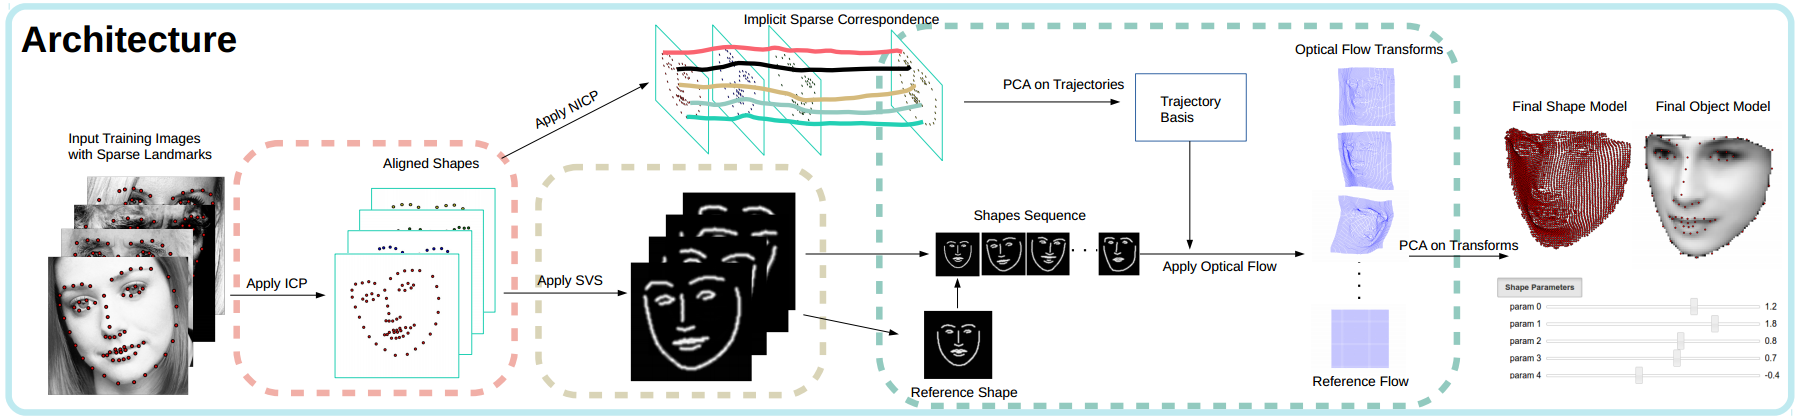
\includegraphics[width=0.5\textwidth]{resources/architecture}
    \caption{Training Architecture}
    \label{fig:archi}
\end{figure}

Deformable models is wildly used for object detection, localization, recognition and tracking while training a deformable model with good generalisation requires tremendous amount of carefully annotated data, which is extremely time consuming. Even more, annotated data normally requires same numbers of landmarks for one object category in every training data that exacerbated the cost of manual annotation. 

In addition, in contrast with sparse landmarks, dense shape reveals more nuanced structure. However, there is, to the best of our knowledge, no available densely annotated data set.

Our research proposed an architecture of accepting various annotations and structuring deformable model without using landmarks. Moreover, we proposed a new method of annotating data which is drawing. The architecture contains two major modules. The first modules handles inconsistent annotation set by converting to landmark independent shape discriminator. While the other module produces shape flow on object discriminators to generate dense flow transformations in shape space following by robust PCA\cite{?} to generate deformable model. In this section, we present the entire architectures, design decision and algorithms.

\subsection{Sparse Landmarks Pre-Processing}
The first module is to bridge the gap that training data has to have consistent number of landmarks. Currently existing annotated databases contains large variety on landmarking, which largely restricted model training to stick to one data set also make evaluation challenging on using distinct data set. We proposed an algorithm that utilizes a combination of Iterative Closest Point and Support Vector Shape for pre-processing before building the model.

\subsubsection{Model Invariance}
The model built should only captures deformations that specific to the object, transformations thus rotation, translation and scaling are processed to be invariant to the model\cite{?}. ICP is applied to align sparse landmarks. ICP is a perfect choice to align various point clouds with no restriction on shape dimension or quantity.

\subsubsection{Landmark Inconsistency}
Ordinarily, construction of deformable model requires training data set having consistent number of landmarks. But unavoidable changes has to be made before applying same algorithm on diverse annotated data set. 

We proposed a method based on Support Vector Shape (SVS)\cite{?}, which is a decision function trained on shapes using v-SVM with RBF kernel. There are several advantages of representing shapes as classifier: general enough to apply on 2D or 3D data, depending on only sparse points and robust against noise, missing data and artifacts. 

Assuming input training images are all differently annotated of same object category. Initially, negative points get randomly sampled around sparse landmarks while annotated landmarks are positive points. Since the number of positive points are far less that the that of negative samples, landmarks are assigned considerably larger weight that $N_p \times W_p=N_n \times W_n$ where $N_p, N_n$ are number of positive/negative points and $W_p, W_n$ are weights of positive/negative samples. 

SVM with RBF kernel function maps any numbers of data points onto an infinite-dimensional space where positive and negative points are linearly separable, hence classification boundary on 2D space represents the actual shape. The decision function for SVM shown below:
\begin{equation} \label{eq:decisionfunc}
    d(x)=\sum_i\alpha k(x_i^*,x)
\end{equation}
where $x_i^*$ are support vectors and $k(x_i^*,x)$ are Gaussian Radial Basis Function kernel $k(x_i^*,x)=exp(-\lambda \|x_i^*,x\|^2)$.

Figure~\ref{fig:build_svs} demonstrate trained shape descriptor using SVM and the final result is irrelevant to landmark amount. Figure~\ref{svs} displays the visualization of the decision function where brighter colour means corresponding pixels belongs to original shape with higher possibility. It is a very generalized shape discriminator that blends inconsistent landmark annotations into decision functions. 


\begin{figure}[h!]
    \centering
    \begin{subfigure}[b]{0.15\textwidth}
            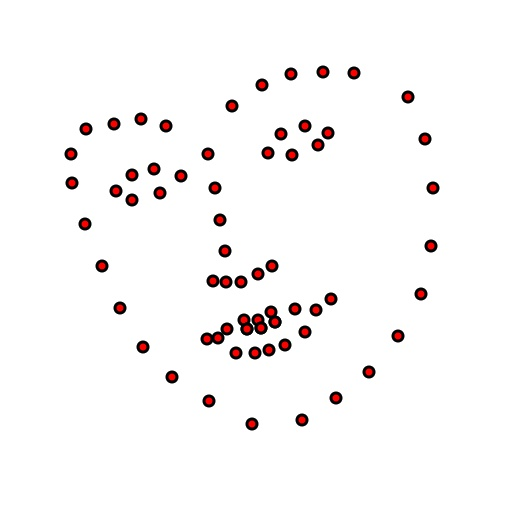
\includegraphics[width=\textwidth]{resources/landmark}
        \caption{Spare landmarks}
    \end{subfigure}
    ~~~~~~~~~
    \begin{subfigure}[b]{0.15\textwidth}
            
\includegraphics[width=\textwidth]{resources/svs}
        \caption{Visualise decision function trained}
        \label{fig:svs}
    \end{subfigure}
    \caption{Decision function trained on sparse landmarks}
    \label{fig:build_svs}
\end{figure}





% ---------------------------------------------------------------------------------------------------------------------------------------------------


\subsection{Shape Flow}

With decision functions built from training data, the second module designed to register all decision functions to mean shape, we named it Shape Flow. Shape Flow is introduced based on optical flow, which generate pixel-wise correspondences for video sequences. Optical flow works for video sequences based on assumptions e.g. brightness constancy and motion smoothness. However, in terms of shapes, neither constant illumination nor continuous motion exists in sequence of shapes as all training data are independent. Thus we proposed shape flow with subspace constrains introduced from trajectories.

\subsubsection{Trajectory Basis} \label{sec:trabasis}
Since shapes from training data set having completely no motion smoothness, it is of importance to contain constrains in optimization on how pixels moves from one shape frame to another. We constrain the optimization on trajectory subspace.
We supervise trajectories from sparse landmarks. To begin with, Non-rigid Iterative Closest Point (NICP)\cite{?} applied on sparse annotated points. NICP deforms target points to fit the template iteratively until all points on target deformed to match points on template. Performs the algorithm for all training data will get an implicit point correlation between sparse shapes.

Since optical flow pixel-wise frame registration, the trajectory basis build should also matches the dimension, which is dense on shapes with trajectory length depends on number of training data. With correspondences produced after applying NICP, Thin-Plate Spline (TPS)\cite{?} transformations are utilized to warp every shape planes to template plane thereby generates an implicit dense shape registering. For all dense transformations $\bm{u_n}(\bm{x}), n \in \{1,...,F\}$, where $F$ is number of data and $\bm{x}$ is vector of pixels, Principle Component Analysis (PCA) is performed on trajectory to obtain low rank trajectory basis:
\begin{equation}
    \begin{bmatrix}
        \bm{u_1}(\bm{x}) \\
        \vdots \\
        \bm{u_F}(\bm{x})
    \end{bmatrix}
    =
    \begin{bmatrix}
        \bm{q_1}(1) & \cdots & \bm{q_R}(1) \\
        \vdots      & \ddots & \vdots  \\
        \bm{q_1}(F) & \cdots & \bm{q_R}(F)
    \end{bmatrix}
    \times
    \begin{bmatrix}
        \bm{v_1}(x) \\
        \vdots \\
        \bm{v_R}(x)
    \end{bmatrix}
\end{equation}
where $\bm{q_i}(n)$ are low rank components with $R \ll 2F$ and $\bm{v_i}(x)$ weighted each component with dependencies on $x$. Simpler expression shown below:
\begin{equation}
    \bm{u_n}(\bm{x})=\sum_{i=1}^R\bm{q_i}(n)\bm{v_i}(x)+\bm{\varepsilon_n}(\bm{x})
\end{equation}
Although optical flow on shapes made under the assumption that objects motion are smooth, the low rank constrain on trajectory basis recovered the hypothesis.

\subsubsection{Algorithm}
To register all decision functions to template shape, decision function $d_i(\bm{x}), i \in {1,...,F}$ are grouped into one sequence before applying flow algorithm. The objective cost function we would like to minimise is:
\begin{align}
    \operatorname*{arg\,min}_{\bm{u_n}(\bm{x}), \bm{v}}&=\alpha \int_{\Omega}\sum_{n=1}^F|\bm{d_n}(x+\bm{u_n}(x))-\bm{d_0}(x)\| dx  \label{eq:costfunc}\\
    &+ \beta \int_{\Omega}\sum_{n=1}^F\|\bm{u_n}(x)-\sum_{i=1}^R\bm{q_i}(n)\bm{v_i}(x)\|^2 dx \label{eq:lowrank}\\
    &+ \sum[\bm{TV}(Qv)]  + v^T.L.v
\end{align}
where $d_n(x)$ is the decision function from~\eqref{eq:decisionfunc}, which returns possibilities of given coordinate classified as shape component where coordianates are from set $\Omega \in \Re^2$. $TV(Qv)$ is total variation as regularization on low rank subspace, $Q$ is trajectory basis and $v^T.L.v$ is low rank spacial constrains.

Term~\eqref{eq:costfunc} state the shape constancy where points having similar classification probability are from same object.
Part~\eqref{eq:lowrank} applies constrain on low rank trajectory basis states in section~\ref{sec:trabasis}.
The objective cost function has two free parameters $u$ and $v$, so we performs alternating minimisation. The equation can be solved using thresholding scheme as used in \cite{?} after linearisation of image functions. The minimisation can be speed up by paralleling the minimisation for every spatial-temporal point $(x;n), x \in \Omega, n \in \{1,...F\}$ independently.

After solving the equation, $\bm{u_n}(\bm{x}), x \in \Omega$ gives a group of deformation fields that registering every decision functions in the shape sequence to reference frame e.g. $\bm{u_1}(\bm{x})$ registers decision function $\bm{d_1}(\bm{x})$ to the reference frame. Figure~\ref{fig:deformationfield} demonstrates deformation fields that warps from reference frame where there is no deformation.

\begin{figure}[h!]
    \centering
        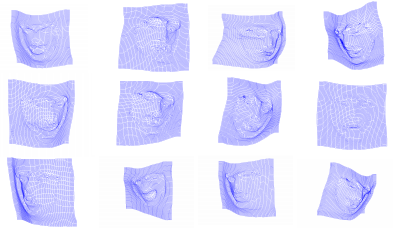
\includegraphics[width=0.5\textwidth]{resources/df}
    \caption{Deformation field built}
    \label{fig:deformationfield}
\end{figure}

Applying PCA on deformations trains dense deformable shape model:
\begin{equation*}
    \bm{s_p}=\bm{\bar{s}} + \bm{U}_s\bm{p}
\end{equation*}
where $\bm{s_p}$ is deformed shape instance. $\bm{\bar{s}}$ is mean shape and $\bm{U}_s\bm{p}$ are eigenvectors with corresponding parameters $p$. Figure~\ref{fig:models} shows an instance of deformed shape and appearance model.
\begin{figure}[h!]
    \centering
        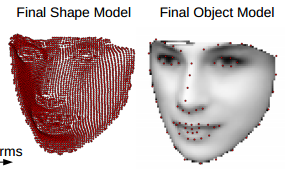
\includegraphics[width=0.4\textwidth]{resources/models}
    \caption{Dense Deformable Model}
    \label{fig:models}
\end{figure}

\subsubsection{Drawing Annotation}

The purpose of the shape descriptor $\bm{d_i}(x)$ generates probabilities for arbitrary points. If we sample points that are exactly pixel-wise integers, and normalise classification value, we can visualise a SVS as an image for example in figure~\ref{fig:svs}. In other words, our architecture will also works for images with landmarks similar to SVS visualisations like drawing. Assuming the intensity of a gray-scale image simulate the decision function, named $\bm{I_i}(x), x \in \Omega, i \in \{1,...F\}$. But in this situation, pixels at image space are discontinued, so $x$ is constrained to be integer and within the view window of size $N\times M$.



\clearpage


%------------------------------------------------------------------------
\section{Evaluation}
    To evaluate the quality of model, 

\subsection{Using Sparse Point Annotation}

\subsection{Using Drawing Annotation}

\clearpage

\section{Conclusion}
    We proposed the first, to the best of our knowledge, methodology that can build a dense deformable model "in-the-wild". This methodology does not require a consistent set of landmarks, avoiding the tedious task of careful manual annotations. We have exploited state-of-the-art multiframe optical flow methodologies to establish accurate and robust dense correspondences among shapes, when represented in a landmarks-free fashion. The experimental evaluations and comparisons revealed that dense AAMs that are built on top of our methodology achieve very good performance and can work effectively even in cases of objects that cannot have consistent landmarks.

\section{Acknowledgement}
    ack


{\small
\bibliographystyle{ieee}
\bibliography{bib}
}


\end{document}
